\section{Make-a-Video}
\label{sec:make_a_video}

Make-a-Video \cite{make_a_video} (2022) by Meta AI is a text-to-video model. Similar to Video-LDM, Make-a-Video extends the text-to-image (T2I) knowledge to diffusion-based text-to-video (T2V) model through spatiotemporally factorized diffusion model. In addition, it doesn't require pairs of text-video data, which allows unsupervised video training, which in turn allows to scale to larger quantities of video data.

They present super-resolution strategies in space and time to generate higher spatial-resolution and higher frame rate video clips, provided a text prompt. They \textbf{leverage image priors} due to the complexity of modeling videos, which simplifies the learning process.







\subsection{Architecture}

\begin{figure}
    \centering
    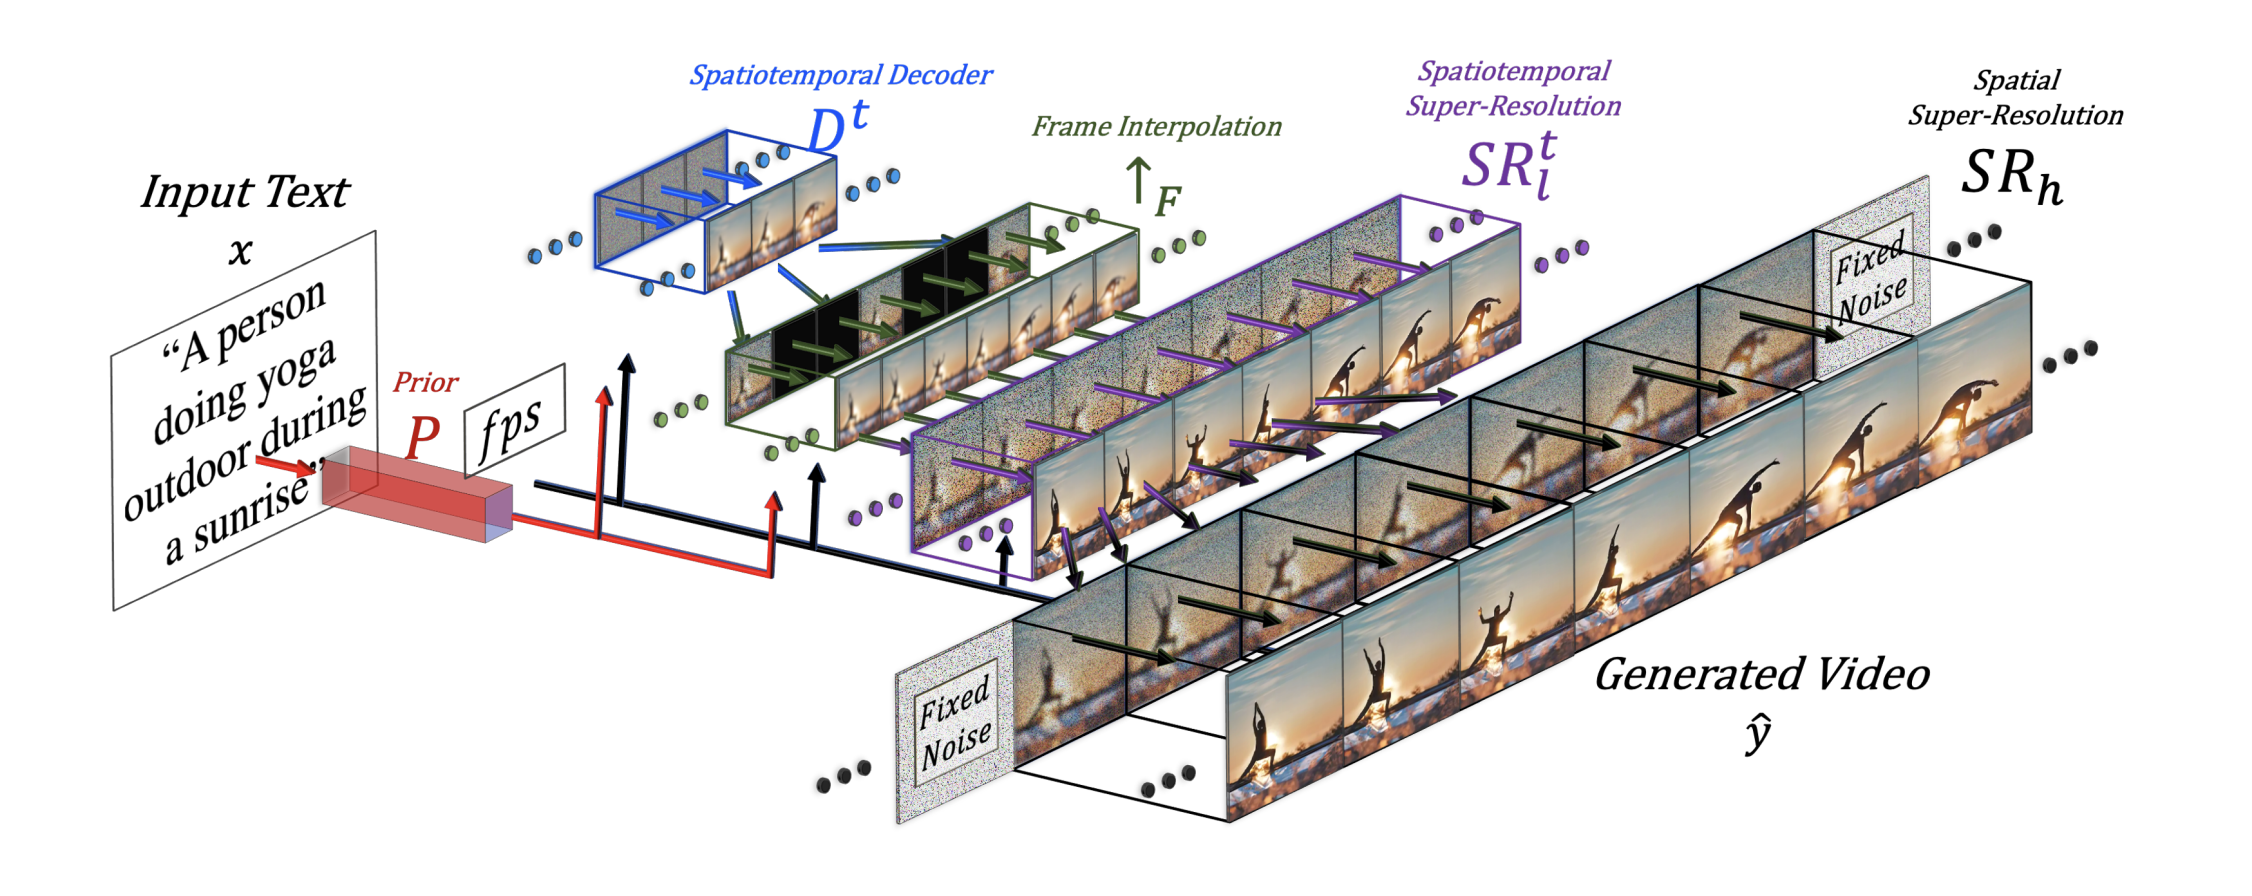
\includegraphics[width=1\textwidth]{images/make_a_video/overview.png}
    \caption{Make-a-Video model high-level architecture overview.}
    \label{fig:make_a_video_overview}
\end{figure}

In figure \ref{fig:make_a_video_overview}, given a text input $x$, its translated into the image embedding prior $P$. The model input is "fps" (frames per second). The \textbf{spatio-temporal decoder $\textcolor{blue}{D^t}$} generates 16 $64\times 64$ frames, which are interpolated into higher fps by the \textbf{frame interpolation model $\textcolor{OliveGreen}{\uparrow_F}$}. Then these frames are increased in spatial resolution to $256\times 256$ by the \textbf{spatiotemporal super-resolution model $\textcolor{Plum}{SR_l^t}$}; and finally increased to resolution $768\times 768$ by \textbf{spatial super-resolution model $SR_h$}. The final output is high-spatiotemporal-resolution video $\hat{y}$.

As discussed above, Make-a-Video has three main components:

\begin{itemize}
    \item Text-to-image model trained on text-image pairs, which is based on the previous work of the OpenAI paper \cite{ramesh2022hierarchical}.
    \item Spatiotemporal convolution and attention layers.
    \item Frame interpolation network $\textcolor{OliveGreen}{\uparrow_F}$.
\end{itemize}

The formal mathematical formulation of the Make-a-Video inference is as follows:

\[ \hat{y_t} = \text{SR}_h \circ \textcolor{Plum}{\text{SR}_l^t} \circ \textcolor{OliveGreen}{\uparrow_F} \circ \textcolor{blue}{D^t} \circ \textcolor{Maroon}{P} \circ \left( \hat{x}, C_x (x) \right) \]

where $x$ is the input text and $C_x$ is the \textbf{CLIP text encoder}.

% TODO: Explain what is \hat{x}  which is BPE-encoded text




\subsection{The T2I model}

The T2I model is based on the core components of the OpenAI paper \cite{ramesh2022hierarchical}. %TODO: Explain in short what this openai paper is about